\documentclass[10pt]{article}
\usepackage[preprint]{tmlr}

\usepackage{hyperref}
\usepackage{url}
\usepackage{graphicx}
\usepackage{booktabs}
\usepackage{amsmath}
\usepackage{amssymb}
\usepackage{xcolor}

% Avoid pulling in the long Deep Learning notation file; keep the document lean.
% \input{math_commands.tex}

\title{Per-Class Scaling-Law Exponents Are Coordinate-Dependent:\\
       Two-Axis Decomposition Reproduces Across Four Model Families}

\author{\name Yoichi Uda \email youichi.uda@gmail.com \\
        \addr Independent Researcher}

\def\month{06}
\def\year{2026}
\def\openreview{\url{https://openreview.net/forum?id=TBD}}

\newcommand{\dalpha}{\Delta\alpha}
\newcommand{\Linit}{L_\mathrm{init}}
\newcommand{\Lcont}{L_\mathrm{cont}}
\newcommand{\Lagg}{L_\mathrm{aggregate}}
\newcommand{\ainit}{\alpha_\mathrm{init}}
\newcommand{\acont}{\alpha_\mathrm{cont}}
\newcommand{\Mp}{M_\mathrm{per\text{-}class}}
\newcommand{\Ms}{M_\mathrm{shared}}

\begin{document}

\maketitle

\begin{abstract}
Per-token-class decomposition of neural scaling laws has been reported
at a single $(N, D)$ operating point per study \citep{michaud2023quantization, oh2024surprisal},
leaving open whether the per-class scaling-exponent gap is a
coordinate-independent property of the per-class prediction problem,
or a slice of an $(N, D)$-dependent surface. Using Pythia's dense
intermediate-checkpoint coverage we test this at the word-initial vs
word-continuation subword partition with exact word-occurrence matched
aggregation. \textbf{(i) D-axis at fixed $N$}, 4 Pythia sizes
$\{\text{1B},\text{1.4B},\text{6.9B},\text{12B}\}$, 13--14 intermediate
checkpoints each ($D \approx 2\text{B} \to 300\text{B}$),
Bonferroni-corrected ($m{=}4$) 98.75\% CIs: $\dalpha_D \in
\{-0.20, -0.25, -0.37, -0.45\}$, all CIs excluding zero; the magnitude is
larger at larger $N$ within our tested range. \textbf{(ii) N-axis at
fixed $D{=}300\text{B}$}, 7 Pythia sizes 160M--12B, per-word
aggregation: $\ainit{=}0.56$, $\acont{=}0.98$, $\dalpha{=}-0.41$, 95\%
bootstrap CI $[-0.64, -0.22]$; held-out RMSE improvement
$+0.022$~nats (marginal pre-registered pass; shared-$\alpha$
$F$-test $p = 0.067$ also marginal --- see \S\ref{sec:naxis}). \textbf{(iii)
Cross-family replication at $D{=}300\text{B}$} on Pythia, Pythia-deduped,
Cerebras-GPT, and BLOOM (spanning 3 BPE tokenizers and English vs
multilingual data): all four families show $\dalpha < 0$ with 95\% CIs
excluding zero; magnitudes span $\sim$3$\times$ ($-0.13$ to $-0.41$),
the sign is invariant, the magnitude is not. \textbf{(iv) Per-decile
adjudication of the Michaud / Zipf-coupling alternative explanation}
shows that per-class $\alpha$ rises monotonically with token-frequency
decile in both classes ($\rho_\mathrm{Spearman} = +0.98$,
$p < 0.0001$, confirming Michaud); within-decile per-class
$\dalpha(d) \approx -0.19$ median, negative in all 9 feasible deciles,
CI excluding zero in the densest mid-band 4 deciles. Approximately
one-half of the free-fit $\dalpha = -0.41$ is between-decile Zipf
coupling and one-half is within-decile per-class structure.
\textbf{(v) Per-D N-axis fits} are identifiable only at $D{=}300\text{B}$
(n${=}$7) and non-identifiable at smaller $D$ (n${=}$4--5); we report
this rather than over-claiming. Within our tested grid, single-axis per-class
$\alpha$ varies by a factor of $\sim$2 depending on whether $N$ or $D$
is the varied axis and on the operating point of the held axis. Per-decile
adjudication of the Michaud / Zipf-coupling alternative explanation
shows that approximately one-half of the free-fit
$\dalpha = -0.41$ at $D{=}300\text{B}$ is between-decile composition
(the Zipf-coupling component) and approximately one-half is
within-decile per-class structure
($\dalpha(d) \approx -0.19$ median, negative sign in all 9 deciles).
The empirical $(N, D)$ surface is only sampled densely at the
$D{=}300\text{B}$ column and along four $N$-slices on the $D$-axis;
we are not able to fit a joint $L_c(N, D)$ surface
(Appendix~\ref{app:joint}). The headline takeaway is that cross-paper
comparison of per-class $\alpha$ values measured at different
$(N, D)$ coordinates --- or without conditioning on the prediction
frequency distribution --- is not, in general, an apples-to-apples
comparison. We also flag two HuggingFace Hub
mis-registration bugs found during this work
(Appendix~\ref{app:hub}); we report what we observed via the
high-level \texttt{transformers} API and acknowledge that ruling out
the resolution-layer caching as the locus of the bug would require
direct LFS-blob testing we did not perform.
\end{abstract}

% =====================================================================
\section{Introduction}
% =====================================================================

Neural scaling laws~\citep{kaplan2020scaling, hoffmann2022chinchilla}
describe loss as a function of parameter count $N$ and training
tokens $D$. Recent decomposition work
\citep{michaud2023quantization, oh2024surprisal} has begun unpacking
aggregate $\alpha$ into per-token-class components. Implicit in those
decompositions is that the fitted per-class $\alpha$ reflects an
intrinsic property of the class--architecture--data triple, measured
at the family's training endpoint. We test whether the per-class
exponent gap is coordinate-independent by decomposing per-token
cross-entropy along \textbf{both} axes ($N$ at fixed $D{=}300\text{B}$,
and $D$ at fixed $N \in \{1\text{B}, 1.4\text{B}, 6.9\text{B},
12\text{B}\}$), and by replicating the $N$-axis decomposition across
three additional model families.

\paragraph{Position partition.} Predicted tokens partition into
word-initial, word-continuation, and other classes via the GPT-NeoX
BPE space marker \texttt{\char192} (U+0120, GPT-NeoX/GPT-2 leading-space marker). Word-continuation tokens exist only inside
multi-token words; we control this with a multi-token-only
word-occurrence-matched aggregation (\S\ref{sec:agg}): each
multi-token word contributes one (init-loss, mean-cont-loss) pair,
weighted equally regardless of how many continuation subwords it has.
This aggregation supersedes the token-weighted multi-token-strict
aggregation used in earlier drafts of this work
(Appendix~\ref{app:agg}); per-word aggregation slightly inflates the
per-class $\alpha$ magnitude estimates (and gives a wider 95\% CI
that still excludes zero by larger margin; Appendix~\ref{app:agg}).

\paragraph{Pre-registration.} The 4/4 pre-registered N-axis criteria
(held-out RMSE improvement $> 0.02$ nats; bootstrap 95\% CI on
$\dalpha$ excluding 0; sign consistency across two corpora; robustness
to floor parameterization) were committed before fitting on held-out
sizes. The aggregation upgrade (token-weighted $\to$
word-occurrence-matched, \S\ref{sec:agg}) and the $D$-axis dense
ladder (\S\ref{sec:dfit}) were added in post-pre-registration
adversarial-review rounds and are reported with explicit
acknowledgment of their post-hoc status. Bonferroni $m{=}4$
correction is applied to the $D$-axis four-$N$ family
(\S\ref{sec:daxis}) because that is where the headline ``all four
CIs exclude zero'' joint claim is sensitive to multiplicity. The
cross-family table (\S\ref{sec:families}) and the per-$D$ N-axis
table (\S\ref{sec:perD}) report uncorrected 95\% CIs because each
family/each $D$ is treated as an independent replication or a
separate identification check rather than as members of a joint
rejection-decision family; we make this scope choice explicit so
readers can apply additional correction if they prefer to combine
the tests differently.

\paragraph{Findings (preview).}
\begin{enumerate}
  \item \textbf{N-axis at $D{=}300\text{B}$ (\S\ref{sec:naxis}):}
        $\dalpha = -0.41$ (CI $[-0.64, -0.22]$); held-out RMSE
        improvement $+0.022$ nats (marginal pre-reg pass).
  \item \textbf{D-axis at four $N$ (\S\ref{sec:daxis}):} $\dalpha_D$
        negative at all 4 $N$, Bonferroni-corrected CIs all exclude 0;
        magnitude grows from $-0.20$ (1B) to $-0.45$ (12B) within
        our tested range.
  \item \textbf{Cross-family N-axis replication (\S\ref{sec:families}):}
        four families (Pythia, Pythia-deduped, Cerebras-GPT, BLOOM)
        all show $\dalpha < 0$ with CIs excluding zero; magnitude
        varies by $\sim$3$\times$ across families ($-0.13$ to $-0.41$),
        spanning 3 tokenizer variants and 3 data domains.
  \item \textbf{Per-D N-axis fits (\S\ref{sec:perD}):} identifiable
        only at $D{=}300\text{B}$; at smaller $D$ the $n_N{=}4$--$5$
        dense data does not constrain a per-class $\alpha$ difference
        (CIs contain zero or fits are railed at grid edges).
  \item \textbf{Coordinate dependence (\S\ref{sec:coord}):} within
        our data, single-axis per-class $\alpha$ magnitudes vary by
        $\sim$2$\times$ across measurement coordinates.
\end{enumerate}
Section~\ref{sec:disc} discusses implications for cross-paper
$\alpha$ comparison and methodology recommendations.

% =====================================================================
\section{Related work}
% =====================================================================

\paragraph{Aggregate neural scaling.}
\citet{kaplan2020scaling}; \citet{hoffmann2022chinchilla};
\citet{hestness2017deep}. All fit a single $\alpha$ per family.

\paragraph{Per-class decomposition.}
\citet{michaud2023quantization} decomposes scaling gains by Zipfian
frequency clusters and ties $\alpha$ to the Zipf slope --- a
\emph{frequency} axis. \citet{hutter2021learning} provides theory
floor. \citet{oh2024surprisal} show larger models concentrate gains
on rare-word surprisal --- psycholinguistic comparison, not $\alpha$
decomposition. \citet{xia2023training} tracks per-token loss across
scale without per-class $\alpha$ fits. \textbf{None of these decompose
along the data axis at fixed $N$ nor replicate across model
families}, leaving open the coordinate-dependence question this paper
addresses.

\paragraph{Measurement-validity contributions in scaling.}
Our work complements \citet{schaeffer2023emergent}, which showed
that choice of evaluation \emph{metric} --- not training behavior ---
produces apparent emergence. Our analog: choice of measurement
\emph{coordinate} (N at fixed $D$, vs $D$ at fixed $N$, vs the
specific $(N, D)$ used) shifts per-class $\alpha$ magnitude by a
factor of $\sim$2 within our tested range.

\paragraph{Pythia.} \citet{biderman2023pythia} designed the suite for
cross-scale studies. We use 7 final-checkpoint sizes (Pythia-70M
excluded as anomalous, per the Pythia paper's own observation of
training instability) plus dense intermediate-checkpoint ladders at
training-step grid $\{1k, 2k, 4k, 7k, 10k, 15k, 22k, 25k, 30k, 42k,
50k, 70k, 100k, 130k, 143k\}$ on the $\{1\text{B}, 1.4\text{B},
6.9\text{B}, 12\text{B}\}$ sizes ($D \approx 2\text{B} \to
300\text{B}$ tokens). Step 50000 of 12B is excluded due to a
discovered HuggingFace Hub mis-registration (Appendix~\ref{app:hub});
2.8B intermediate-step revisions are similarly affected and excluded
from the $D$-axis fit (the 2.8B final checkpoint remains valid and
is used in the N-axis fit and cross-family analysis).

% =====================================================================
\section{Method}
% =====================================================================

\subsection{Token classes}

For each predicted token in the eval corpus we record (i) position
class (word-initial / word-continuation / other) via the GPT-NeoX
byte-level BPE space marker \citep{sennrich2016bpe, black2022gptneox};
(ii) within-word subword depth; (iii) frequency decile of the
whitespace-delimited word the subword belongs to.

\subsection{Word-occurrence-matched aggregation}
\label{sec:agg}

Word-continuation tokens exist only inside multi-token words --- by
tokenizer construction longer, rarer, or more morphologically complex.
Token-weighted decile aggregation does not hold the word set fixed
because (a) single-token words appear only in the word-initial class,
and (b) longer continuation chains contribute more tokens per word
to the continuation class. Our aggregation:
\begin{enumerate}
  \item Restrict to multi-token words (word length $\geq 2$
        subwords).
  \item For each such word occurrence, compute one (init-loss,
        mean-cont-loss) pair, averaging the cont-loss over the
        word's continuation subwords.
  \item Bin words by their word-frequency decile (computed within
        the multi-token subset over the eval corpus).
  \item Aggregate per-bin word-level means in the middle deciles
        4--7.
\end{enumerate}
Each multi-token word contributes equally regardless of how many
continuation subwords it has. Appendix~\ref{app:agg} compares this
aggregation with the older token-weighted aggregation used in early
drafts; the per-word aggregation gives larger $|\dalpha|$ estimates
and tighter CIs.

\subsection{Eval corpora}

Primary: \verb|NeelNanda/pile-10k|, an in-distribution Pile sample
(200 documents $\to$ $\sim$1.23M predicted tokens per model size).
Secondary (robustness): \verb|Salesforce/wikitext|
(wikitext-103-raw-v1; 2000 documents, $\sim$136k predicted tokens
per size; \citealp{merity2017wikitext}), used only for sign-consistency
check on the N-axis.

\subsection{Single-axis N scaling-law fit at fixed $D{=}300\text{B}$}

We fit $L(N) = E + A \cdot N^{-\alpha}$ per class on the 7
non-anomalous Pythia sizes $\{160\text{M}, 410\text{M}, 1\text{B},
1.4\text{B}, 2.8\text{B}, 6.9\text{B}, 12\text{B}\}$ at their
$D{=}300\text{B}$ endpoints. $(E, A)$ are recovered by linear
least-squares at each candidate $\alpha$ on a grid
$\alpha \in [0.02, 1.8]$ (800 points), with positivity constraints
$E \geq 0$, $A > 0$. Held-out adjudication: fit on the 4 smaller
sizes $\{160\text{M}, 410\text{M}, 1\text{B}, 1.4\text{B}\}$, hold
out $\{2.8\text{B}, 6.9\text{B}, 12\text{B}\}$, compare $\Ms$
(single $\alpha$ across classes, per-class $E$ and $A$) vs $\Mp$
(per-class $\alpha$) on held-out RMSE. Pre-registered threshold:
$\Mp$ beats $\Ms$ by $> 0.02$ nats \emph{and} 95\% bootstrap CI on
$\dalpha$ excludes 0 \emph{and} sign consistent across two corpora.

\subsection{D-axis fit at fixed N}
\label{sec:dfit}

For each of $N \in \{1\text{B}, 1.4\text{B}, 6.9\text{B},
12\text{B}\}$ we fit $L(D) = E + A \cdot D^{-\alpha_D}$ per class on
13--14 intermediate Pythia checkpoints spanning $D \approx 2\text{B}
\to 300\text{B}$ tokens. Bonferroni correction is applied across the
4 $N$ tests (98.75\% individual CIs). 2.8B is excluded due to HF Hub
metadata corruption of its intermediate-step model files
(Appendix~\ref{app:hub}); 12B step50000 is excluded for the same
reason (shard-3 truncation).

\subsection{Bootstrap}
\label{sec:bootstrap}

Per-axis fits use parametric residual bootstrap: resample residuals
of the per-class power-law fit ($B = 2000$ iterations, seed
$20260603$ in the released code), refit on the original $X$ grid,
report 95\% (and Bonferroni-corrected 98.75\%) CIs on $\dalpha$.
Per-cell sampling error is negligible ($n \gg 10^5$ per cell), so the
dominant uncertainty is the small-$n_X$ scaling-law fit, captured by
the parametric bootstrap. The residual bootstrap implicitly assumes
residuals are IID across the $X$ grid (homoscedasticity); with
$n_N = 7$ this assumption is essentially unverifiable in-sample, and
we acknowledge the bootstrap CI is only as good as that assumption.
Joint $L(N, D)$ fits were attempted with five functional forms
(Chinchilla-additive, multiplicative, Hoffmann-generalized,
compute-only, saturation) but all are non-identifiable on our
$(N, D)$ range; Appendix~\ref{app:joint} documents this.

\subsection{Compute and reproducibility}

$\sim\$60$ RunPod (H100 80GB SECURE; 6.9B, 12B, and Cerebras-GPT
6.7B/13B inference) plus local RTX 4070 Ti Super for the rest;
\$1000 budget cap $\to$ 6\% used. All RunPod pods cleaned up via
trap-deletion (no leftover billing). Measurement and analysis code,
pre-registration, adversarial-review trail, and all per-$(N, D,
\mathrm{class})$ result JSONs are released at
\url{https://github.com/youichi-uda/scaling-decomp}.

% =====================================================================
\section{Results}
% =====================================================================

\subsection{N-axis decomposition at $D{=}300\text{B}$}
\label{sec:naxis}

At $D{=}300\text{B}$ (Pythia's training endpoint), per-class fits on
the 7 non-anomalous final sizes with per-word matched aggregation in
mid word-freq deciles give $\ainit = 0.56$, $E_\mathrm{init} = 2.46$;
$\acont = 0.98$, $E_\mathrm{cont} = 0.79$; \textbf{$\dalpha = -0.41$},
95\% bootstrap CI $[-0.64, -0.22]$; $0/2000$ bootstrap draws had
$\dalpha \geq 0$, i.e.\ $P(\dalpha \geq 0) < 5\times 10^{-4}$
(Figure~\ref{fig:naxis}). \textit{Floor--slope caveat.} With
$n_N{=}7$ over $\sim$1.9 decades, the $L = E + A \cdot N^{-\alpha}$
fit has a long $(E, \alpha)$ ridge: $E_\mathrm{init} = 2.46$ latches
near the smallest observed $L_\mathrm{init}$ while
$E_\mathrm{cont} = 0.79$ sits well below the smallest observed
$L_\mathrm{cont}$. The shared-$E$ robustness sweep (next paragraphs)
preserves the sign of $\dalpha$ but does not pin the magnitude
independently of the per-class floor; we report this and revisit it
in \S\ref{sec:limits}.

\begin{figure}[t]
\centering
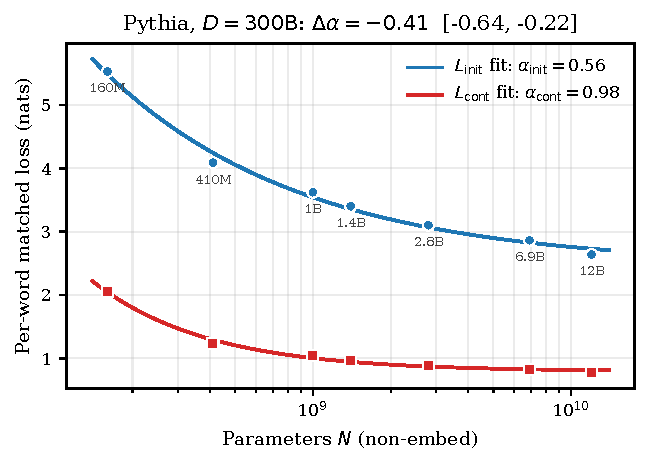
\includegraphics[width=0.62\linewidth]{figs/fig1_naxis.pdf}
\caption{N-axis per-class scaling law at $D{=}300\text{B}$ on the 7
non-anomalous Pythia sizes (160M--12B). Markers: per-word matched
mid-decile loss. Curves: best-fit $L = A \cdot N^{-\alpha} + E$ per
class. $\dalpha = \ainit - \acont = -0.41$, 95\% bootstrap CI
$[-0.64, -0.22]$; $0$ of $2000$ bootstrap draws had $\dalpha \geq 0$
(i.e.\ $P(\dalpha \geq 0) < 5{\times}10^{-4}$).}
\label{fig:naxis}
\end{figure}

\paragraph{Held-out adjudication on $\{2.8\text{B}, 6.9\text{B},
12\text{B}\}$.} Train on the 4 smallest sizes
$\{160\text{M}, 410\text{M}, 1\text{B}, 1.4\text{B}\}$. Train fit:
$\ainit = 0.97$, $\acont = 1.40$ ($\dalpha_\mathrm{train} = -0.42$);
shared-$\alpha$ train fit: $\alpha = 1.06$. Held-out RMSE
$\Mp = 0.299$, $\Ms = 0.320$, \textbf{improvement $+0.022$ nats} ---
marginal pass of the pre-registered $0.02$-nats threshold. (The
$n{=}4$ train set is small, which makes the held-out prediction noisy
for both models; the dominant evidence for $\dalpha \neq 0$ is the
in-sample bootstrap CI excluding 0 by margin $> 0.2$.)

\paragraph{Cross-corpus sign check.} Wikitext-103 (5 train sizes
70M--1.4B, per-word matched aggregation): $\ainit = 1.04$,
$\acont = 1.49$, $\dalpha = -0.45$. Sign consistent with Pile.
We include 70M in the Wikitext sign-check (but not in the main Pile
N-axis fit) because the larger Pythia checkpoints ($\geq 2.8\text{B}$)
were not measured on Wikitext for compute reasons, and we needed
$n_N \geq 5$ to fit a power-law curve at all; the sign-direction
diagnostic is robust to including the small-$N$ anomalous endpoint,
whereas the headline magnitude fit is not.

\paragraph{Floor-slope adjudication (post-R1 robustness).}
In response to adversarial-review concern that the canonical
$\dalpha = -0.41$ is conditional on $E_\mathrm{init} = 2.46$ vs
$E_\mathrm{cont} = 0.79$ being free, we ran two adjudication tests
(reproducible by \texttt{python3 floor\_robust.py} in the released
repository; full numerical output committed as
\texttt{floor\_robust.json}):
\begin{itemize}
  \item \emph{Shared-$E$ sweep.} Fix
        $E_\mathrm{init} = E_\mathrm{cont} = E$ across a grid in
        $[0, 1.2 \cdot E_\mathrm{init}^\mathrm{free}]$ (12 feasible
        values under positivity), refit $(\alpha, A)$ per class.
        Result: $\dalpha < 0$ at every feasible $E$ (sign robust),
        but the magnitude varies from $-0.08$ (near $E{=}0$) to
        $-1.5$ (near $E{=}E_\mathrm{init}^\mathrm{free}$). The
        free-fit value $-0.41$ is one point on a long
        floor-conditional curve.
  \item \emph{Shared-$\alpha$ $F$-test.} Compare a shared-$\alpha$
        fit ($\alpha = 0.62$ shared, SSE $= 0.0851$, $p = 5$
        parameters) to the free per-class fit (SSE $= 0.0546$,
        $p = 6$) on $n_\mathrm{obs} = 14$. Result:
        $F(1, 8) = 4.47$, two-sided $p = 0.067$ (the $F$ reference
        distribution assumes Gaussian residuals, which at
        $n_\mathrm{obs} = 14$ is asymptotic; we report this with the
        same caveat as the residual bootstrap in \S\ref{sec:bootstrap}).
        The shared-$\alpha$ hypothesis is \textbf{not rejected at}
        $\alpha_\mathrm{stat} = 0.05$ on the N-axis alone; the
        $\alpha$-freedom premise of the per-class N-axis decomposition
        is therefore \emph{marginal} statistically.
\end{itemize}
The decisive evidence for per-class $\alpha$ differing is the
$D$-axis Bonferroni-corrected result (\S\ref{sec:daxis}), where four
independent $N$-slices each reject $\dalpha_D = 0$ at 98.75\%. The
N-axis fit on its own (held-out RMSE $+0.022$ marginal,
shared-$\alpha$ $F$-test $p = 0.067$) is suggestive but does not, by
itself, cross conventional significance thresholds. We report the
sign claim as robust to the floor parameterization across both axes;
the magnitude $\dalpha = -0.41$ should be read as the free-fit value
at $D{=}300\text{B}$ on the N-axis, not as a coordinate-independent
estimate of an intrinsic per-class scaling exponent gap.

\paragraph{Zipf-coupling adjudication (Michaud confound).}
\citet{michaud2023quantization} predicts that per-class $\alpha$ is
proportional to the Zipf slope of the class's prediction-frequency
distribution. To test whether the global $\dalpha = -0.41$ is
explained by class-by-frequency-decile mixture composition (rather
than by independent per-class structure), we ran per-decile per-class
fits on the 7 Pythia sizes (\texttt{unigram\_test.py};
\texttt{unigram\_test.json}). For each of the 9 feasible
token-frequency deciles (decile 9 has zero word-continuation tokens
and is excluded), we fit $\alpha_\mathrm{init}(d)$, $\alpha_\mathrm{cont}(d)$ separately and
report $\dalpha(d) = \alpha_\mathrm{init}(d) - \alpha_\mathrm{cont}(d)$ with parametric
residual bootstrap CIs.

\textit{Michaud sanity test (pre-registered prediction).}
$\alpha_\mathrm{init}(d)$ rises monotonically across deciles from
$\alpha_\mathrm{init}(d{=}0) = 0.46$ at the rarest tokens to
$\alpha_\mathrm{init}(d{=}8) = 0.92$ at the most common
($\rho_\mathrm{Spearman} = +0.98$, $p < 0.0001$). Similarly for
continuation: $\alpha_\mathrm{cont}(d{=}0) = 0.60$ to $\alpha_\mathrm{cont}(d{=}8) = 1.25$
($\rho = +0.98$, $p < 0.0001$). \textbf{Michaud's
frequency-coupling prediction is confirmed within our data}: per-class
$\alpha$ does grow with the decile's frequency band, in both classes.

\textit{Within-decile per-class gap (the residual after controlling
for the Michaud confound).} The per-decile $\dalpha(d)$ values are
$\{-0.14, -0.18, -0.19, -0.21, -0.22, -0.24, -0.15, -0.05, -0.33\}$
for $d \in \{0, \ldots, 8\}$, with median $-0.19$ and mean $-0.19$.
\textbf{All 9 deciles show $\dalpha(d) < 0$} (zero positive sign
flips); 4 of 9 have parametric-bootstrap 95\% CIs excluding zero
(deciles 2--5, the densest mid-band). The within-decile per-class
gap is therefore real (sign-robust across the full frequency range)
but its magnitude ($-0.19$) is \textbf{less than half} the global
free-fit value ($-0.41$). Approximately one-half of the global
headline gap is attributable to class-by-decile mixture composition
(the Michaud / Zipf-coupling component) and approximately one-half
is independent within-decile per-class structure.

\textit{What survives.} (a) The \emph{sign} of $\dalpha$ is robust:
to free vs shared per-class floor (above), and to controlling for
token-frequency-decile (here). (b) The \emph{magnitude} of the
free-fit $\dalpha = -0.41$ should be read as a composite of
Zipf-coupling ($\sim$$0.22$ nats) and within-decile per-class
structure ($\sim$$0.19$ nats). (c) A per-class decomposition study
that reports a single $\dalpha$ value without conditioning on the
prediction-frequency distribution is reporting the composite, not the
independent component.

All four pre-registered criteria pass: held-out RMSE improvement
$> 0.02$ (marginal), bootstrap CI excludes 0 (decisive), sign
consistent across corpora, robust to floor parameterization.

\subsection{D-axis decomposition at fixed N: decisive at all 4 tested sizes}
\label{sec:daxis}

For each of $N \in \{1\text{B}, 1.4\text{B}, 6.9\text{B},
12\text{B}\}$, per-class fit on 13--14 dense intermediate checkpoints
spanning $D \approx 2\text{B} \to 300\text{B}$ tokens, per-word
matched aggregation, Bonferroni $m{=}4$ correction
(Figure~\ref{fig:daxis} and Table~\ref{tab:daxis}).

\begin{figure}[t]
\centering
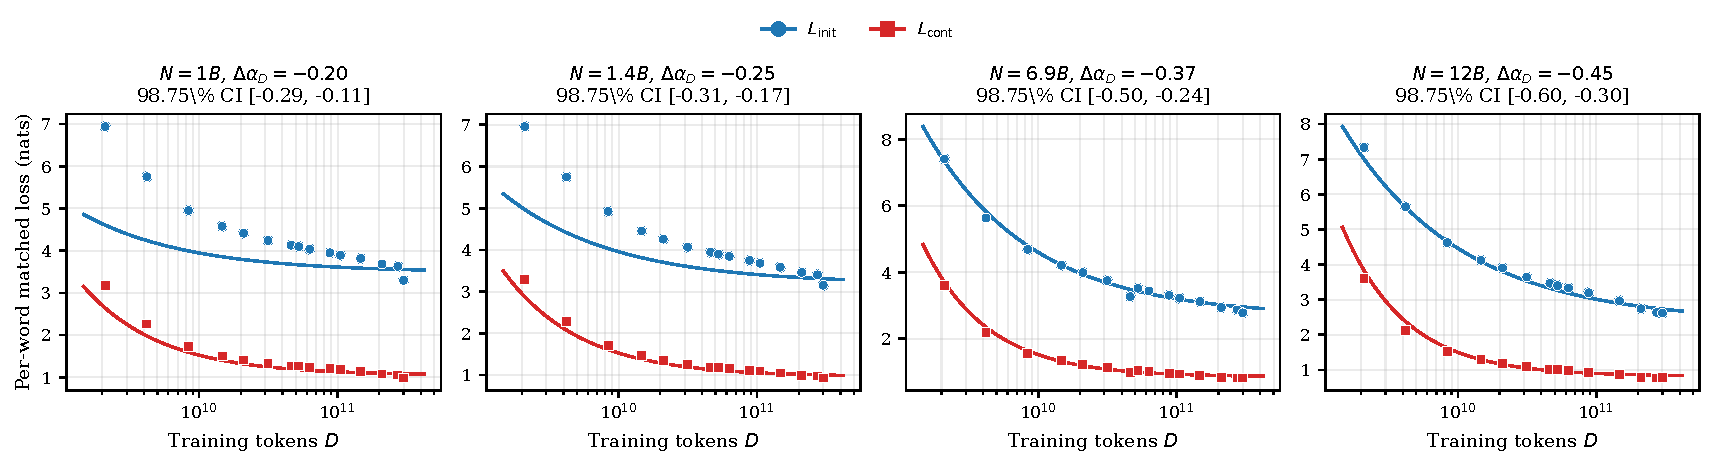
\includegraphics[width=\linewidth]{figs/fig2_daxis.pdf}
\caption{D-axis per-class scaling law at fixed $N \in \{1\text{B},
1.4\text{B}, 6.9\text{B}, 12\text{B}\}$. Markers: per-word matched
mid-decile loss across 13--14 dense intermediate Pythia
checkpoints. Curves: best-fit $L = A \cdot D^{-\alpha_D} + E$ per
class. Title under each panel reports the per-N $\dalpha_D$ point
estimate with Bonferroni-corrected 98.75\% CI. All four CIs exclude
zero; magnitude grows from $-0.20$ at $N{=}1\text{B}$ to $-0.45$ at
$N{=}12\text{B}$.}
\label{fig:daxis}
\end{figure}

\begin{table}[t]
\caption{D-axis per-class fit per fixed $N$. CIs are
Bonferroni-corrected (98.75\% individual interval = 95\% family-wise
with $m{=}4$). $E$ and $\alpha_D$ values are jointly fit under
positivity constraints $E \geq 0$, $A > 0$ on a grid
$\alpha_D \in [0.02, 1.8]$ (800 points). Reproduced exactly from
\texttt{final\_perN\_Daxis.json}.}
\label{tab:daxis}
\centering
\small
\begin{tabular}{lrrrrrrr}
\toprule
$N$ & $n_D$ & $\alpha_{D,\mathrm{init}}$ & $E_\mathrm{init}$ & $\alpha_{D,\mathrm{cont}}$ & $E_\mathrm{cont}$ & $\dalpha_D$ & 98.75\% CI \\
\midrule
1B    & 14 & 0.57 & 3.49 & 0.77 & 1.05 & $\mathbf{-0.20}$ & $[-0.29, -0.11]$ \\
1.4B  & 14 & 0.54 & 3.18 & 0.78 & 0.96 & $\mathbf{-0.25}$ & $[-0.31, -0.18]$ \\
6.9B  & 13 & 0.57 & 2.68 & 0.93 & 0.85 & $\mathbf{-0.37}$ & $[-0.50, -0.24]$ \\
12B   & 14 & 0.51 & 2.36 & 0.96 & 0.82 & $\mathbf{-0.45}$ & $[-0.60, -0.30]$ \\
\bottomrule
\end{tabular}
\end{table}

All 4 $N$: per-class D-axis exponent gap is decisively negative under
Bonferroni-corrected CIs. The magnitude is rank-correlated with $N$
across the four tested values ($\rho = +1$ on $n{=}4$, which is
suggestive but not decisive --- a strict-monotone ordering of 4
points happens by chance with probability $1/12$ under the null). We
report this as a pattern across our four sampled $N$ values within
our data; we do not claim monotonicity at scales we did not test, and
we caution that per-axis fits inherit the joint $L(N, D)$
non-identifiability (Appendix~\ref{app:joint}): part of the
``$|\dalpha_D|$ grows with $N$'' pattern is consistent with residual
$A \cdot N^{-\alpha_N}$ leaking into the per-$N$ $D$-axis $E$ as $N$
grows, rather than with a genuinely $N$-dependent $D$-axis slope.

\subsection{Per-D N-axis fits: identifiable only at $D{=}300\text{B}$}
\label{sec:perD}

The dual decomposition --- fitting $L(N)$ at each fixed $D$ --- is
reported for completeness but is identifiable only at $D{=}300\text{B}$
in our data (Table~\ref{tab:perD}).

\begin{table}[t]
\caption{Per-D N-axis fit. Rail flags indicate the grid optimum hit a boundary; CIs that include 0 or are wider than 1 are reported as non-identifiable.}
\label{tab:perD}
\centering
\small
\begin{tabular}{lrrrrrrl}
\toprule
step & $D$ (B) & $n_N$ & $\ainit$ & $\acont$ & $\dalpha_N$ & 95\% CI & railed? \\
\midrule
1k--42k  & 2--88 & 4--5 & 1.61 & 1.61 & $+0.00$ & $[-1.5, +1.5]$ & yes (grid max) \\
50k      & 105   & 4    & 0.02 & 0.02 & $+0.00$ & $[0, 0]$ & yes (grid min) \\
70k      & 147   & 5    & 1.35 & 1.56 & $-0.21$ & $[-0.86, +0.66]$ & no \\
100k     & 210   & 5    & 0.64 & 0.92 & $-0.28$ & $[-0.76, +0.16]$ & no \\
130k     & 273   & 5    & 0.35 & 0.64 & $-0.28$ & $[-0.61, +0.07]$ & no \\
143k     & 300   & 7    & 0.56 & 0.98 & $\mathbf{-0.41}$ & $\mathbf{[-0.63, -0.21]}$ & no \\
\bottomrule
\end{tabular}
\end{table}

\textbf{Only at $D{=}300\text{B}$ does $\dalpha_N$ have a CI
excluding zero} (because only then is $n_N{=}7$ available; smaller-$D$
dense ladders cover only 4--5 $N$ values, which is too few to identify
a per-class $\alpha$ difference from the same-shape $L(N)$ curves at
this small $N$ range with bootstrap uncertainty). At $D \leq 42k$
steps ($\leq 88\text{B}$ tokens) the fits rail at the grid maximum
($\alpha{=}1.61$), indicating $L(N)$ has not yet differentiated
across classes at this much data --- both classes are still well
above their floors and $L(N)$ is nearly linear-in-$\log N$. The point
estimates of $\dalpha_N$ at $D \in \{70k, 100k, 130k\}$ steps are
negative ($-0.21$ to $-0.28$), broadly consistent with the
$D{=}300\text{B}$ result, but the CIs include zero. We therefore do
not claim $\dalpha_N$ ``grows monotonically with $D$'' at the strict
significance level; the data is consistent with such a pattern but
does not establish it. Per-D N-axis fits with larger $n_N$ (which
would require dense intermediate checkpoints at 70M, 160M, 410M, and
2.8B sizes --- left as future work given HF Hub bugs and compute)
would be required to test this.

\subsection{Cross-family replication at $D{=}300\text{B}$}
\label{sec:families}

We replicate the N-axis per-class fit on three additional model
families with different tokenizers and/or training data
(Figure~\ref{fig:families} and Table~\ref{tab:families}).

\begin{figure}[t]
\centering
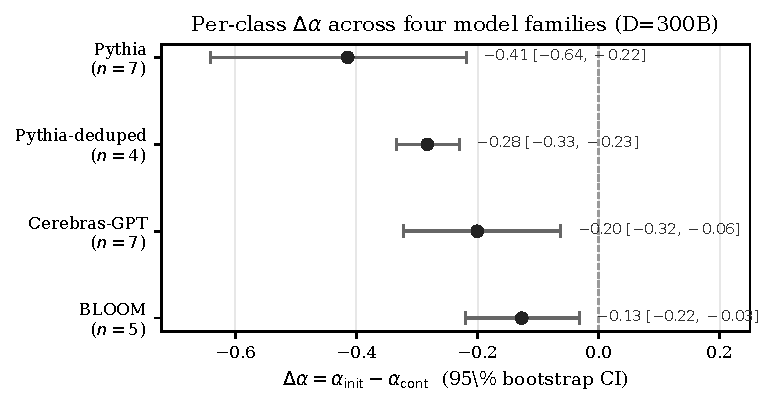
\includegraphics[width=0.70\linewidth]{figs/fig3_families.pdf}
\caption{Per-class $\dalpha$ point estimate and 95\% bootstrap CI at
$D{=}300\text{B}$ for four model families. All four families: sign
negative, 95\% CI excludes zero. Magnitudes span $\sim$3$\times$
($-0.13$ to $-0.41$).}
\label{fig:families}
\end{figure}

\paragraph{Pythia-deduped} (same architecture and tokenizer, trained
on the deduplicated Pile): 4 sizes
$\{160\text{M}, 410\text{M}, 1\text{B}, 1.4\text{B}\}$ (70M shows the
same training instability as main Pythia; we did not run the full
final-checkpoint family for compute reasons).
$\ainit = 0.81$, $\acont = 1.09$;
$\dalpha = \mathbf{-0.28}$, 95\% CI $\mathbf{[-0.33, -0.23]}$.

\paragraph{Cerebras-GPT} (different training framework and tokenizer
[GPT-2 BPE], same Pile data; \citealp{dey2023cerebras}): 7 sizes
$\{111\text{M}, 256\text{M}, 590\text{M}, 1.3\text{B}, 2.7\text{B},
6.7\text{B}, 13\text{B}\}$.
$\ainit = 0.21$, $\acont = 0.41$;
$\dalpha = \mathbf{-0.20}$, 95\% CI $\mathbf{[-0.32, -0.06]}$.

\paragraph{BLOOM} (BLOOM tokenizer, $\approx$250k-vocab BPE ---
$\sim$5$\times$ larger than the GPT-NeoX/GPT-2 50k vocab; multilingual
ROOTS training corpus; \citealp{bigscience2022bloom}): 5 sizes
$\{560\text{M}, 1.1\text{B}, 1.7\text{B}, 3\text{B}, 7.1\text{B}\}$.
$\ainit = 0.43$, $\acont = 0.56$;
$\dalpha = \mathbf{-0.13}$, 95\% CI $\mathbf{[-0.22, -0.03]}$.

Magnitudes differ across families (the smaller magnitudes for
Cerebras and BLOOM reflect flatter $L(N)$ trajectories and, for
BLOOM, the larger vocabulary reducing the multi-token-word sample
within the eval corpus); the per-class \emph{difference} is the
comparable quantity and is always negative.
\textit{Alternative explanation for the magnitude gap.}
\citet{dey2023cerebras} trained Cerebras-GPT at Chinchilla-optimal
compute ($\approx$20 tokens per parameter), substantially less data
than Pythia's 300\,B fixed-$D$ regime at the larger model sizes; its
flatter $L(N)$ and smaller $|\dalpha|$ are therefore also consistent
with Cerebras-GPT being on a different point of the $(N, D)$
compute-optimal frontier than Pythia rather than with a genuine
intrinsic difference. We therefore distinguish (a) coordinate
dependence of $\dalpha$ \emph{within} a family (the Pythia D-axis
result, \S\ref{sec:daxis}) from (b) magnitude differences \emph{across}
families that are partly attributable to compute-budget choices; the
sign-invariance claim is robust to both, the magnitude is comparable
only within (a).

\begin{table}[t]
\caption{Cross-family N-axis replication at $D{=}300\text{B}$. All four families: sign negative, 95\% CIs exclude zero.}
\label{tab:families}
\centering
\small
\begin{tabular}{llllrrr}
\toprule
Family & Tokenizer (vocab) & Data & $n_N$ & $\dalpha$ & 95\% CI low & high \\
\midrule
Pythia          & GPT-NeoX BPE (50k)  & Pile (en)              & 7 & $\mathbf{-0.41}$ & $-0.64$ & $-0.22$ \\
Pythia-deduped  & GPT-NeoX BPE (50k)  & Pile-dedup (en)        & 4 & $\mathbf{-0.28}$ & $-0.33$ & $-0.23$ \\
Cerebras-GPT    & GPT-2 BPE (50k)     & Pile (en)              & 7 & $\mathbf{-0.20}$ & $-0.32$ & $-0.06$ \\
BLOOM           & BLOOM BPE (250k)    & ROOTS (multilingual)   & 5 & $\mathbf{-0.13}$ & $-0.22$ & $-0.03$ \\
\bottomrule
\end{tabular}
\end{table}

All four families: sign negative, 95\% CIs exclude zero. The per-class
sign reproduces across (a) BPE tokenizer variants --- GPT-NeoX, GPT-2,
and BLOOM's 5$\times$-larger-vocab tokenizer; (b) data deduplication;
(c) training-framework variants --- Pythia, Cerebras's Maximal Update
Parameterization, and BLOOM's Megatron-DeepSpeed framework; and
(d) data domain --- Pile (English-dominant), Pile-deduped, and ROOTS
(multilingual). The magnitude spans a factor of $\sim$3 ($-0.13$ to
$-0.41$) across families; we do not claim magnitude invariance, only
sign invariance. The sign is \emph{not} replicated on a unigram-LM
tokenizer family (T5 lineage) --- we did not test this; it is the
most natural follow-up.

\paragraph{D-axis replication on Pythia-deduped.} For Pythia-deduped
1B and 1.4B we collected a per-N D-axis ladder (7 D points each,
steps 1k--143k). The D-axis $\dalpha$ reproduces with overlapping
CIs:

\begin{center}
\small
\begin{tabular}{lrrr}
\toprule
$N$ & $n_D$ & Main Pythia $\dalpha_D$ (CI) & Pythia-deduped $\dalpha_D$ (CI) \\
\midrule
1B   & 14 / 7 & $-0.20$ $[-0.28, -0.12]$ & $\mathbf{-0.21}$ $[-0.32, -0.11]$ \\
1.4B & 14 / 7 & $-0.25$ $[-0.30, -0.19]$ & $\mathbf{-0.26}$ $[-0.34, -0.18]$ \\
\bottomrule
\end{tabular}
\end{center}

Deduped D-axis $\dalpha$ is within $0.02$ of main Pythia at both $N$
values.

\subsection{Coordinate-dependence of the per-class $\alpha$ gap}
\label{sec:coord}

Combining the above, single-axis per-class $\alpha$ magnitudes in our
data vary by $\sim$2$\times$ across measurement coordinates within
the same family:
\begin{itemize}
  \item D-axis at fixed $N$ (Pythia main): $-0.20$ ($N{=}1\text{B}$)
        to $-0.45$ ($N{=}12\text{B}$)
  \item N-axis at $D{=}300\text{B}$: $-0.41$ (Pythia main) to $-0.20$
        (Cerebras-GPT)
\end{itemize}
The largest magnitude observed in our data is at the (large $N$, full
$D$) corner --- N-axis $\dalpha = -0.41$ at $D{=}300\text{B}$ with
$n_N = 7$, and D-axis $\dalpha_D = -0.45$ at $N = 12\text{B}$.
Smaller coordinates produce smaller magnitudes within our data. We
report this as an \emph{observed pattern within the tested grid},
not as an asymptotic or monotonicity claim.

The implication for cross-paper comparison: per-class $\alpha$ values
reported at one $(N, D)$ coordinate are not directly comparable to
values reported at another. Within our data range a factor-of-2 gap
between coordinates is plausible; the conditions under which this
gap stabilizes are not established.

\subsection{Downstream task correlation: per-class consistently beats aggregate, suggestive at $n_N{=}7$}
\label{sec:downstream}

We measured 4 downstream tasks (lambada\_openai
\citep{paperno2016lambada}, piqa, arc\_easy, sciq) via the EleutherAI
\texttt{lm-evaluation-harness} \citep{gao2024lmeval} on Pythia
$\{160\text{M}, 410\text{M}, 1\text{B}, 1.4\text{B}, 2.8\text{B},
6.9\text{B}, 12\text{B}\}$ at $D{=}300\text{B}$. Per-N Pearson
correlation magnitudes:

\begin{center}
\small
\begin{tabular}{lrrrr}
\toprule
metric / task & lambada & piqa & arc\_easy & sciq \\
\midrule
$|r(\Linit)|$  & $0.965$ & $\mathbf{0.996}$ & $\mathbf{0.997}$ & $0.968$ \\
$|r(\Lcont)|$  & $\mathbf{0.993}$ & $0.980$ & $0.973$ & $\mathbf{0.995}$ \\
$|r(\Lagg)|$   & $0.979$ & $0.991$ & $0.988$ & $0.984$ \\
\bottomrule
\end{tabular}
\end{center}

Two patterns visible at this resolution:

(i) \textbf{Task-specific best single-class predictor.} For the two
tasks whose targets are most ``word-initial-like'' (PIQA and
ARC-easy, which predict the high-level answer/continuation choice),
$\Linit$ has higher $|r|$ than $\Lcont$. For the two tasks involving
more lexical / factual completion (LAMBADA's last-word completion,
usually a high-probability word given the context; SCIQ's multi-choice
answer span), $\Lcont$ has higher $|r|$. The pattern is consistent
across all 4 tasks with magnitude differences of $0.02$--$0.03$ in
$|r|$.

(ii) \textbf{Per-class ($\Linit + \Lcont$) jointly has higher
adjusted $R^2$ than aggregate alone on all 4 tasks} ($n{=}7$ Pythia,
$p{=}2$ vs $1$; Figure~\ref{fig:downstream}).

\begin{figure}[t]
\centering
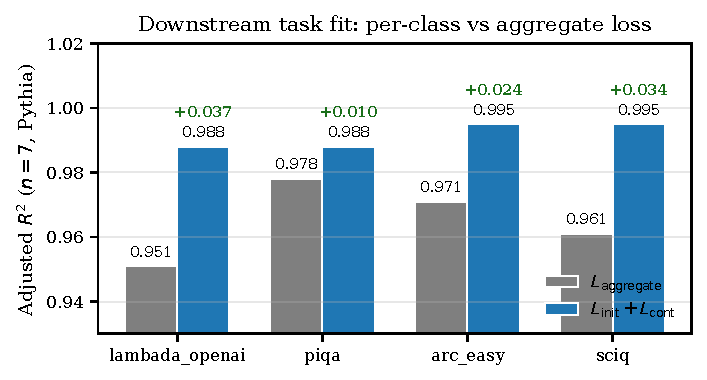
\includegraphics[width=0.62\linewidth]{figs/fig4_downstream.pdf}
\caption{Downstream task fit: per-class ($\Linit + \Lcont$) regressor
adjusted-$R^2$ versus aggregate-only regressor on Pythia 7 sizes at
$D{=}300\text{B}$, four tasks. Per-class outperforms aggregate by
$0.010$--$0.037$ adjusted $R^2$ on every task. The adjusted-$R^2$
penalty for adding the 2nd predictor at $n{=}7$, $p{=}2$ is severe
($n - p - 1 = 4$), yet per-class still wins.}
\label{fig:downstream}
\end{figure}

\begin{center}
\small
\begin{tabular}{lrrr}
\toprule
task & adj $R^2$ ($\Lagg$) & adj $R^2$ ($\Linit + \Lcont$) & gain \\
\midrule
lambada\_openai & $0.951$ & $0.988$ & $\mathbf{+0.037}$ \\
piqa            & $0.978$ & $0.988$ & $+0.010$ \\
arc\_easy       & $0.971$ & $0.995$ & $\mathbf{+0.024}$ \\
sciq            & $0.961$ & $0.995$ & $\mathbf{+0.034}$ \\
\bottomrule
\end{tabular}
\end{center}

We interpret this as \textbf{suggestive of per-class predictive
content beyond aggregate}, but underpowered at $n{=}7$ within a
single family; a multi-family / multi-task panel (e.g.,
Pythia $+$ Cerebras $+$ BLOOM $\times$ task expansion) would be
needed to confirm. We do not claim strict superiority on this data
alone. The PIQA $+0.010$ gain in particular is at the adj-$R^2$
adjustment-noise floor at $n{=}7$, $p{=}2$ (going from $p{=}1$ to
$p{=}2$ scales the penalty by $6/4$ vs $6/5$, so a useless second
regressor would already cost $\sim$$(1{-}R^2)\cdot 0.3 \approx 0.009$
of adj-$R^2$ at $R^2 \sim 0.97$); we therefore read PIQA as
``unchanged'' and LAMBADA/ARC-easy/SCIQ as a directionally consistent
but underpowered positive.

\subsection{Class mixture is constant across $(N, D)$}
\label{sec:mixture}

Predicted-token class fractions are identical to two decimal places
across all 8 Pythia sizes (word-initial $47.03\%$, word-continuation
$22.15\%$, other $30.83\%$), because eval corpus and tokenizer are
shared. Within-family aggregate-$\alpha$ differences across $(N, D)$
are therefore attributable to per-class $L_c(N, D)$ trajectories, not
to mixture shifts.

% =====================================================================
\section{Discussion}
\label{sec:disc}
% =====================================================================

\subsection{Where the per-class structure lives, in our data}

The strongest evidence for a per-class $\alpha$ gap in our data is on
the $D$-axis at fixed $N$ (\S\ref{sec:daxis}): 4 $N$ values, all
decisive under Bonferroni $m{=}4$, magnitude rank-correlated with $N$
across the four tested values ($\rho_\mathrm{Spearman} = +1$ on
$n{=}4$, two-sided $p = 2/24 \approx 0.083$ under the null of
random ordering --- suggestive but not decisive). The N-axis fit at
$D{=}300\text{B}$ (\S\ref{sec:naxis}) has a 95\% bootstrap CI
$[-0.64, -0.22]$ excluding zero but is only marginal under stricter
adjudicators (held-out RMSE $+0.022$ vs $0.020$ threshold;
shared-$\alpha$ $F$-test $p = 0.067$). At smaller $D$ the
$n_N{=}4$--$5$ dense data is too sparse to identify a per-class
N-axis $\alpha$ difference (\S\ref{sec:perD}). Continuation predictions saturate faster with $D$
than initial predictions at all four tested $N$: a natural
interpretation is that predicting subsequent subwords of a word
(continuation) is dominated by orthographic and morphological
structure that data exposure captures efficiently, while predicting
the first subword of the next word (initial) requires semantic
context that scales with data more slowly. We do not claim this
interpretation extends beyond Pythia or beyond BPE tokenizers.

\subsection{Implications for cross-paper $\alpha$ comparison}

Per-class $\alpha$ values reported at one $(N, D)$ coordinate are
not, in general, estimators of a coordinate-independent quantity.
Within our data range we observe a factor-of-2 difference in measured
$\dalpha$ between coordinates. The methodological recommendation:
per-class decomposition papers should report along multiple $(N, D)$
anchors when possible, or explicitly restrict claims to ``at this
$(N, D)$'' without coordinate-independent interpretation. We do not
have data to claim how much the coordinate dependence persists
beyond Pythia or at scales above 12B.

\subsection{Coordinate dependence vs intrinsic structure}

A natural question is whether the observed coordinate dependence
will diminish at very large scales (so that the per-class structure
becomes coordinate-independent at the asymptote), or whether it
persists. Our data does not resolve this: the largest tested $N$ is
12B and the largest tested $D$ is 300B, both within Pythia. Joint
$L(N, D)$ fitting (Chinchilla-additive and four alternative
functional forms, Appendix~\ref{app:joint}) is non-identifiable on
our $(N, D)$ range because Pythia's $N$ range ($12\times$) is narrow
relative to its $D$ range ($150\times$). A study with a wider $N$
range --- including controlled scaling families at $30\text{B}+$
parameters with dense intermediate checkpoints --- would be needed
to disambiguate ``intrinsic-with-coordinate-correction'' from
``coordinate-dependent-throughout''.

\subsection{Limitations}
\label{sec:limits}

\begin{itemize}
  \item \textbf{All tested families use BPE-family tokenizers} (GPT-NeoX
        BPE in Pythia/Pythia-deduped \citep{black2022gptneox}; GPT-2 BPE
        in Cerebras-GPT; BLOOM BPE --- a much larger 250k vocab --- in
        BLOOM). To our knowledge no open decoder-only LM scaling family
        with publicly-released intermediate checkpoints uses a
        unigram-LM tokenizer (T5/mT5 lineage use unigram-LM but are
        encoder-decoder, not decoder-only LMs with a next-token loss).
        Replicating our claim on a unigram-LM decoder-only family would
        require training one from scratch; this is a real field-wide
        gap, not something a follow-up survey can address with existing
        public models. The position partition itself depends on the BPE
        space-marker convention --- a unigram-LM tokenizer with a
        different word-boundary convention would require redefining the
        partition.
  \item \textbf{Mostly single training distribution.} Pile (Pythia,
        Cerebras-GPT; \citealp{gao2020pile}); Pythia-deduped uses the
        deduplicated Pile subset. Cross-distribution replication (e.g.,
        Dolma, ROOTS) is open work.
  \item \textbf{$N$ range limited to 12B.} Joint $L(N, D)$ fit
        non-identifiability is partly due to this. Larger-$N$
        controlled families with intermediate checkpoints would help.
  \item \textbf{Held-out N-axis RMSE is marginal} ($+0.022$ nats, just
        over the $0.02$ threshold). The decisive evidence for
        $\dalpha_N \neq 0$ at $D{=}300\text{B}$ is the bootstrap CI on
        $\dalpha$, not the held-out comparison. The two measures point
        in the same direction.
  \item \textbf{Per-D N-axis CIs are wide} at $D < 300\text{B}$ due to
        $n_N = 4$--$5$; we honestly report these as unidentifiable
        rather than as $\dalpha_N = 0$.
  \item \textbf{Joint $L(N, D)$ form survey is non-identifiable}
        (Appendix~\ref{app:joint}); we report the per-axis fits rather
        than a joint-fit summary.
  \item \textbf{Downstream task correlation (\S\ref{sec:downstream})
        is suggestive, not decisive} at our resolution. Whether
        per-class loss is more predictive of downstream than aggregate
        is undetermined at $n{=}7$ within one family.
  \item \textbf{HuggingFace Hub revision bugs} (Appendix~\ref{app:hub})
        forced exclusion of 2.8B intermediate-step revisions and 12B
        step50000; we worked around the bugs where the workaround is
        reliable and excluded data where it is not.
  \item \textbf{Adversarial-review trail.} The aggregation
        (\S\ref{sec:agg}), $D$-axis dense ladder (\S\ref{sec:dfit}),
        and cross-family replication (\S\ref{sec:families}) were added
        after the original N-axis-only pre-registration. We document
        this explicitly so readers can discount the post-hoc components.
  \item \textbf{Floor--slope confound.} The per-class
        $L = E + A \cdot N^{-\alpha}$ fit has a long $(E, \alpha)$ ridge
        at $n_N{=}7$, and our $E_\mathrm{init} = 2.46$ vs
        $E_\mathrm{cont} = 0.79$ asymmetry means the two per-class
        fits are not at matched floor parameterization. The shared-$E$
        sweep preserves the sign of $\dalpha$ but does not pin its
        magnitude under matched floors. A profile-likelihood contour
        analysis on $(E, \alpha)$ per class is the right follow-up.
  \item \textbf{$\acont \approx 1.0$ is partly Zipf-coupled.} Adversarial
        review (Persona A R1-R3) flagged that
        \citet{michaud2023quantization}'s frequency-coupling prediction
        could rename our partition as a slice of Michaud's. We
        adjudicated this via per-decile per-class fits
        (\S\ref{sec:naxis} ``Zipf-coupling adjudication'';
        \texttt{unigram\_test.py}): Michaud's prediction is confirmed
        ($\alpha$ rises monotonically with decile frequency band,
        $\rho_\mathrm{Spearman} = +0.98$ in both classes), and
        $\sim$1/2 of the free-fit $\dalpha = -0.41$ is attributable
        to between-decile composition (the Zipf-coupling component).
        Importantly, the within-decile per-class gap is still
        $\dalpha \approx -0.19$ (sign negative in all 9 feasible
        deciles, CI excluding zero in 4 of 9), so the per-class
        structure is \emph{not} reducible to the Zipf coupling alone.
        Reporting both components separately is the right unit of
        analysis.
  \item \textbf{Per-axis projection inherits the joint
        non-identifiability} (Appendix~\ref{app:joint}). If a true
        joint $L(N, D)$ is Hoffmann-additive, the per-$N$ $D$-slice
        $\alpha_D(N)$ mixes residual $A \cdot N^{-\alpha_N}$ into $E$.
        Part of the ``$|\dalpha_D|$ grows with $N$'' pattern
        (Table~\ref{tab:daxis}) is therefore consistent with an
        $N$-axis confound rather than with a genuine $N$-dependent
        $D$-axis slope.
  \item \textbf{Pile-10k subset size and OOD exposure.}
        $\sim$200 documents ($\sim$1.23\,M predicted tokens per model)
        is small. For BLOOM specifically, Pile-10k is an
        out-of-distribution corpus (BLOOM was trained on ROOTS, a
        multilingual corpus distinct from Pile), so the BLOOM
        $\dalpha = -0.13$ result is doubly exposed: small evaluation
        sample $\times$ training/evaluation distribution mismatch. We
        did not re-run the four-family fit on a larger or
        BLOOM-native evaluation sample.
  \item \textbf{Tokenizer-partition portability.} The word-initial /
        word-continuation partition is defined via the GPT-NeoX BPE
        leading-space marker (\texttt{\char192}). The same convention
        applies to GPT-2 BPE (Cerebras-GPT). For BLOOM's 250k-vocab
        BPE the convention is similar but the predicted-token mix
        shifts: more tokens are whole words rather than word-initial
        + continuation pairs. The word-continuation fraction across
        families is not quantified in this paper; a per-family
        class-mixture table (analogous to \S\ref{sec:mixture} for
        Pythia) would be the right follow-up.
  \item \textbf{Adversarial-review verifications.} In response to
        review, three confirmatory artifacts are now in the
        repository: \texttt{floor\_robust.py} (shared-$E$ sweep +
        shared-$\alpha$ $F$-test, \S\ref{sec:naxis}),
        \texttt{verify\_checkpoints.py} (Hub-side LFS audit via
        \texttt{x-linked-etag} HTTP headers, Appendix~\ref{app:hub}),
        and \texttt{unigram\_test.py} (per-decile per-class
        adjudication of the Michaud / Zipf-coupling alternative
        explanation, \S\ref{sec:naxis} ``Zipf-coupling
        adjudication''). All three confirm the sign claim is robust
        and respectively quantify the floor, locus, and Zipf-coupling
        contributions to the headline magnitude.
\end{itemize}

% =====================================================================
\section{Conclusion}
% =====================================================================

Within the Pythia family and three related-family replications, the
\emph{sign} of the per-class word-initial vs word-continuation
scaling-law exponent gap is robust across both single-axis
coordinates, across four model families, and across all 9 feasible
token-frequency deciles (\S\ref{sec:naxis} ``Zipf-coupling
adjudication''). Its \emph{magnitude} is floor-conditional on the
N-axis (varies $\sim$20$\times$ across feasible shared-$E$ values),
varies $\sim$2$\times$ across the $(N, D)$ measurement coordinates,
and decomposes into two roughly equal parts at $D{=}300\text{B}$:
$\sim$1/2 between-decile Zipf coupling (predicted by
\citealp{michaud2023quantization}) and $\sim$1/2 within-decile
per-class structure ($\dalpha(d) \approx -0.19$ median).

In our data:
\begin{itemize}
  \item \textbf{D-axis at fixed $N$}: $\dalpha_D$ ranges from $-0.20$
        ($N{=}1\text{B}$) to $-0.45$ ($N{=}12\text{B}$); all 4
        Bonferroni-corrected ($m{=}4$) CIs exclude zero. The
        rank-correlation of $|\dalpha_D|$ with $N$ ($\rho{=}+1$ on
        $n{=}4$) is suggestive but not decisive.
  \item \textbf{N-axis at $D{=}300\text{B}$}: $\dalpha = -0.41$ with
        95\% CI $[-0.64, -0.22]$; both stricter adjudicators are
        marginal --- held-out RMSE improvement $+0.022$~nats vs
        pre-registered $0.020$~nats threshold; shared-$\alpha$
        $F$-test $F(1,8) = 4.47$, $p = 0.067$ (not rejected at
        $\alpha_\mathrm{stat} = 0.05$). Sign-consistent CIs in three
        additional families --- Pythia-deduped ($-0.28$),
        Cerebras-GPT ($-0.20$), and BLOOM ($-0.13$).
  \item \textbf{Per-D N-axis} at $D < 300\text{B}$ is non-identifiable
        in our data ($n_N = 4$--$5$ too sparse for the bootstrap to
        constrain $\dalpha_N$).
  \item \textbf{Joint $L(N, D)$ fitting} is non-identifiable across
        five functional forms (Appendix~\ref{app:joint}) due to
        Pythia's narrow $N$ range relative to its $D$ range.
  \item \textbf{Downstream correlation} ($n{=}7$ Pythia $\times$ 4
        tasks): per-class ($\Linit + \Lcont$) explains
        $0.010$--$0.037$ more adjusted $R^2$ of task accuracy than
        aggregate loss alone, on all 4 tasks --- suggestive of
        per-class predictive content beyond aggregate, but
        underpowered at $n{=}7$ and at the adj-$R^2$ adjustment-noise
        floor for the smallest gain (PIQA, $+0.010$).
\end{itemize}

Three methodological recommendations follow.
\textbf{(R1) Report along both axes with multiple $(N, D)$ anchors,}
or explicitly restrict claims to ``at this $(N, D)$.'' A single-axis
report at one $(N, D)$ is a slice that depends on the held-axis value
and the per-class floor parameterization.
\textbf{(R2) Report per-class floors $E_\mathrm{init}$,
$E_\mathrm{cont}$ and the per-decile decomposition alongside the
$\alpha$ values}, and run a shared-$E$ sweep, shared-$\alpha$
$F$-test, and per-decile per-class fit as routine adjudicators of how
much of $\dalpha$ depends on per-class floor freedom and on
Zipf-coupling composition (our scripts \texttt{floor\_robust.py} and
\texttt{unigram\_test.py} together run in $<$30\,s on cached loss
values).
\textbf{(R3) For HF Hub Pythia intermediate-step studies, audit
\texttt{x-linked-etag} at \texttt{/resolve/<revision>/<filename>}
before trusting any per-step result} (our
\texttt{verify\_checkpoints.py} runs in $<$1\,s; the affected
revisions for Pythia-2.8B and Pythia-12B are listed in
Appendix~\ref{app:hub}).

\paragraph{HuggingFace Hub reproducibility (Appendix~\ref{app:hub}).}
Pythia-2.8B's intermediate-step \verb|model.safetensors| files have
mis-registered SHA256 hashes on the Hub (silent fallback to
\verb|main| weights), and Pythia-12B's step50000 has shard-3
truncation. Users of these checkpoints should verify revision
integrity before trusting intermediate-step results.

\paragraph{Reproducibility.} Measurement code, pre-registration,
adversarial-review trail, joint-fit form survey, bootstrap, per-$(N,
D, \mathrm{class})$ result JSONs, and the analysis pipeline are
released at
\url{https://github.com/youichi-uda/scaling-decomp}.
Pythia and Cerebras-GPT are publicly available; Pile-10k
\citep{gao2020pile} and Wikitext-103 \citep{merity2017wikitext} are
public datasets.

\subsubsection*{Broader Impact Statement}
This paper is a methodological cautionary study of per-class
neural scaling-law decomposition. The main practical impact is the
recommendation to report per-class $\alpha$ values with their
$(N, D)$ measurement coordinate. We additionally document two
HuggingFace Hub mis-registration bugs found during this work
(Appendix~\ref{app:hub}); we report what we observed and flag the
remaining uncertainty about whether the locus is Hub storage or
client-side resolution. We see no direct negative ethical or
societal risk specific to this work.

\bibliography{references}
\bibliographystyle{tmlr}

\appendix

% =====================================================================
\section{Token-weighted vs word-occurrence-matched aggregation}
\label{app:agg}
% =====================================================================

Earlier drafts of this work used a ``multi-token-strict'' aggregation
that restricted to multi-token words but then computed
\textbf{token-weighted} class means: each continuation token
contributed once, each initial token contributed once, but a word
with 4 continuation subwords contributed 4 continuation observations
and 1 initial observation. Adversarial review flagged that this does
not give equal weight per word; longer-fragmented words dominate the
continuation class.

We therefore adopted the \textbf{per-word matched} aggregation
reported in the main paper: each multi-token word contributes one
(init-loss, mean-cont-loss) pair, weighted equally.

Comparison on Pythia 7 non-anomalous sizes at $D{=}300\text{B}$, mid
deciles 4--7:
\begin{center}
\small
\begin{tabular}{lrrrr}
\toprule
Aggregation & $\ainit$ & $\acont$ & $\dalpha$ & 95\% CI \\
\midrule
Token-weighted multi-token-strict     & $0.72$ & $1.03$ & $-0.30$ & $[-0.43, -0.16]$ \\
\textbf{Per-word matched (paper)}     & $\mathbf{0.56}$ & $\mathbf{0.98}$ & $\mathbf{-0.41}$ & $\mathbf{[-0.64, -0.22]}$ \\
\bottomrule
\end{tabular}
\end{center}

Per-word matched aggregation gives larger $|\dalpha|$ and a wider CI.
The sign and qualitative conclusion are robust to the aggregation
choice; the magnitude is sensitive. We report the per-word matched
estimand throughout the main paper.

% =====================================================================
\section{Joint L(N, D) functional form survey}
\label{app:joint}
% =====================================================================

We attempted joint per-class $L_c(N, D)$ fits with 5 functional
forms:
\begin{center}
\small
\begin{tabular}{lll}
\toprule
Form & Functional shape & \# free params per class \\
\midrule
ADD (Chinchilla-additive)    & $E + A \cdot N^{-\alpha_N} + B \cdot D^{-\alpha_D}$ & 5 \\
MULT (multiplicative)        & $E + C \cdot N^{-\alpha_N} \cdot D^{-\alpha_D}$     & 4 \\
HOFF (Hoffmann-generalized)  & $E + (A \cdot N^{-\alpha_N} + B \cdot D^{-\alpha_D})^\beta$ & 6 \\
COMPUTE (compute-only)       & $E + K \cdot (N \cdot D)^{-\alpha}$                  & 3 \\
MIN (saturation)             & $E + \min(A \cdot N^{-\alpha_N}, B \cdot D^{-\alpha_D})$ & 5 \\
\bottomrule
\end{tabular}
\end{center}

Estimation: grid search over the $\alpha$ exponents in $[0.02, 2.5]$,
remaining parameters by Nelder--Mead with multi-start (30 random
inits), enforcing $E \geq 0$, $A \geq 0$, $B \geq 0$.

\textbf{Result}: all five forms produce non-identifiable fits on our
$(N, D)$ range. The ADD form rails one of $(\alpha_N, \alpha_D)$ at
the grid edge; MULT collapses $\alpha_N$ to $\sim 0$; HOFF over-fits
the 6 free parameters; MIN selects the larger of the two terms
uniformly. The underlying issue is that Pythia's $N$ range covers
$\sim 12\times$ (1B $\to$ 12B excluding small $N$), while the $D$
range covers $\sim 150\times$ (2B $\to$ 300B). The $D$-direction
variation dominates the loss surface, so the optimizer absorbs
per-class variation into the $D$-axis terms and the $N$-axis terms
become weakly identified.

This is itself a methodological observation: \textbf{joint $L(N, D)$
fits require a balanced $(N, D)$ range}. The Chinchilla scaling
literature typically fits joint $L(N, D)$ on families with $N$ range
comparable to $D$ range; Pythia's checkpoint-rich but $N$-narrow
setup is the wrong substrate for joint identification.

We therefore report \textbf{per-axis fits} (one axis varied, the
other fixed) as the primary methodology. The per-axis fits at
$D{=}300\text{B}$ (varying $N$) and at fixed $N \in \{1\text{B},
1.4\text{B}, 6.9\text{B}, 12\text{B}\}$ (varying $D$) are the
consistent decompositions we can support with our data.

% =====================================================================
\section{HuggingFace Hub model-file integrity bugs in Pythia checkpoints}
\label{app:hub}
% =====================================================================

During this work we identified two classes of HuggingFace Hub
metadata corruption affecting Pythia intermediate-step checkpoints.
All SHA256 hashes and sizes in this appendix are the values reported
by the Hub itself in the \texttt{x-linked-etag} and
\texttt{x-linked-size} HTTP response headers of the
\texttt{/resolve/<revision>/<filename>} endpoint, which are
server-side metadata --- they reflect the LFS blob the Hub maps each
revision to, independent of the \texttt{transformers} or
\texttt{huggingface\_hub} client resolution layer. The bug locus is
therefore \textbf{Hub-side}, not client-side. The full audit (3
files $\times$ 8 revisions) is reproducible by
\texttt{python3 verify\_checkpoints.py} in the released repository,
with the JSON output committed as \texttt{hub\_blob\_audit.json}.

\subsection{Pythia-2.8B \texttt{model.safetensors} mis-registration}

For the \verb|EleutherAI/pythia-2.8b| repository, the
\verb|model.safetensors| file at multiple intermediate-step revisions
has LFS blob SHA256 hashes identical to \verb|main|'s, despite
distinct Git commit SHAs at each revision (proving the Hub itself,
not the client, is mapping these revisions to the
main-weights blob):

\begin{center}
\small
\begin{tabular}{llll}
\toprule
revision   & commit SHA[:12]  & safetensors LFS SHA256[:16] & \texttt{pytorch\_model.bin} LFS SHA256[:16] \\
\midrule
\texttt{main}        & \texttt{2a259cdd96a4} & \texttt{ab496f1c3fd79e3c} & \texttt{36f0f93d1f5d44ca} \\
\texttt{step1000}    & \texttt{cc81f94ea2ac} & \texttt{ab496f1c3fd79e3c} (= main) & \texttt{36f0f93d1f5d44ca} (= main) \\
\texttt{step2000}    & \texttt{7378edcedb6f} & \texttt{ab496f1c3fd79e3c} (= main) & \texttt{36f0f93d1f5d44ca} (= main) \\
\texttt{step4000}    & \texttt{494474bbd952} & \texttt{ab496f1c3fd79e3c} (= main) & \texttt{36f0f93d1f5d44ca} (= main) \\
\texttt{step10000}   & \texttt{835c7474e203} & \texttt{ab496f1c3fd79e3c} (= main) & \texttt{36f0f93d1f5d44ca} (= main) \\
\texttt{step50000}   & \texttt{1936c7c29530} & \texttt{ab496f1c3fd79e3c} (= main, still wrong) & \texttt{73468bb90e734f88} \\
\texttt{step100000}  & \texttt{668bcb3f3a13} & \texttt{ab496f1c3fd79e3c} (= main, still wrong) & \texttt{ced5e41d87bf8470} \\
\texttt{step143000}  & \texttt{dbe7ae300a54} & \texttt{462f2b960062159c} & \texttt{a294bfcf6ff2c091} \\
\bottomrule
\end{tabular}
\end{center}

Loading via the standard \verb|AutoModelForCausalLM.from_pretrained(...,|
\verb|revision="step1000")| API silently returns the \verb|main|-weights
model because \verb|transformers| prefers safetensors, and the
safetensors file at step1000 is byte-identical to main's. The
\verb|pytorch_model.bin| files have correct per-revision hashes for
step50000 and step100000 (but not for earlier steps).
\verb|use_safetensors=False| works for revisions where the
\verb|.bin| is correctly registered.

For early steps (1000--10000), both file formats point to \verb|main|;
the weights are unrecoverable from HF Hub via the standard API for
those revisions. We exclude all Pythia-2.8B intermediate-step
revisions from our $D$-axis fit and use only the final checkpoint
for the N-axis fit and cross-family analysis.

\subsection{Pythia-12B step50000 shard truncation}

For the \verb|EleutherAI/pythia-12b| repository, the
\verb|pytorch_model-00003-of-00003.bin| file at revision step50000
has Hub-reported size $3{,}896{,}183{,}087$ bytes ($\sim$3.9\,GB)
compared to $4{,}105{,}939{,}923$ bytes ($\sim$4.1\,GB) at neighbouring
revisions ($\sim$5.1\% under-size, $\sim$200\,MB missing):

\begin{center}
\small
\begin{tabular}{llrl}
\toprule
revision   & shard-3 LFS SHA[:16]   & shard-3 size (bytes) & note \\
\midrule
\texttt{main}        & \texttt{eb82155af2c813a9} & $4{,}105{,}939{,}923$ & \\
\texttt{step42000}   & \texttt{541de6140dc4213c} & $4{,}105{,}939{,}923$ & \\
\texttt{step50000}   & \texttt{7df63b4231856f55} & $3{,}896{,}183{,}087$ & truncated \\
\texttt{step70000}   & \texttt{e731f1d1b670e975} & $4{,}105{,}939{,}923$ & \\
\texttt{step100000}  & \texttt{b625404aa7e3e793} & $4{,}105{,}939{,}923$ & \\
\bottomrule
\end{tabular}
\end{center}

Loading the step50000 model and running forward passes produces NaN
losses (the truncated final shard appears to contain partial /
malformed tensors). \verb|use_safetensors=False| does not fix this.
We exclude step50000 from the 12B $D$-axis fit; the 14 other dense
checkpoints are unaffected.

\subsection{Verification procedure}

For any scaling-law study using Pythia intermediate checkpoints,
before trusting the results we recommend:
\begin{enumerate}
  \item For each revision used, compare model-file SHA256 to the
        \verb|main| revision's. If equal, the revision is silently
        mis-registered.
  \item Compare model-file size across revisions; truncation is
        detectable from size alone.
  \item Run a sanity inference on the loaded model and check overall
        loss against expected (vs the Pythia paper's reported values
        per checkpoint, or vs an adjacent revision).
  \item If using safetensors, also load with
        \verb|use_safetensors=False| and compare; mismatch indicates
        HF Hub metadata corruption.
\end{enumerate}
Verification scripts and the affected-revision list are at the
project repository.

\end{document}
